%=======================================================================================
%  Reduced Order Models - Notes 
%
%=======================================================================================
\documentclass[11pt]{article}
% \usepackage[bookmarks=true]{hyperref}  % this changes the page location !
\usepackage[bookmarks=true,colorlinks=true,linkcolor=blue]{hyperref}

% \input documentationPageSize.tex
\hbadness=10000 
\sloppy \hfuzz=30pt

% \voffset=-.25truein
% \hoffset=-1.25truein
% \setlength{\textwidth}{7in}      % page width
% \setlength{\textheight}{9.5in}    % page height

\usepackage{calc}
\usepackage[lmargin=.75in,rmargin=.75in,tmargin=.75in,bmargin=.75in]{geometry}


\input homeHenshaw

\usepackage{tikz}

\input trimFig.tex

% The amssymb package provides various useful mathematical symbols
\usepackage{amsmath}
\usepackage{amssymb}

\newcommand{\Largebf}{\sffamily\bfseries\Large}
\newcommand{\largebf}{\sffamily\bfseries\large}
\newcommand{\largess}{\sffamily\large}
\newcommand{\Largess}{\sffamily\Large}
\newcommand{\bfss}{\sffamily\bfseries}
\newcommand{\smallss}{\sffamily\small}

\newcommand{\beq}{\begin{equation}}
\newcommand{\eeq}{\end{equation}}
\newcommand{\Omegav}{\boldsymbol{\Omega}}
\newcommand{\omegav}{\boldsymbol{\omega}}

\newcommand{\phiv}{\boldsymbol{\phi}}
\newcommand{\psiv}{\boldsymbol{\psi}}

\input wdhDefinitions.tex
\newcommand{\mbar}{\bar{m}}
\newcommand{\Rbar}{\bar{R}}
\newcommand{\Ru}{R_u}         % universal gas constant
% \newcommand{\grad}{\nabla}
\newcommand{\Div}{\grad\cdot}

\newcommand{\alphav}{\boldsymbol{\alpha}}
\newcommand{\betav}{\boldsymbol{\beta}}

\newcommand{\tauv}{\boldsymbol{\tau}}
\newcommand{\sigmav}{\boldsymbol{\sigma}}
\newcommand{\thetav}{\boldsymbol{\theta}}
\newcommand{\kappav}{\boldsymbol{\kappa}}
\newcommand{\lambdav}{\boldsymbol{\lambda}}
\newcommand{\xiv}{\boldsymbol{\xiv}}
\newcommand{\sumi}{\sum_{i=1}^n}


\newcommand{\Bc}{\mathcal{B}}
\newcommand{\Cc}{\mathcal{C}}
\newcommand{\Dc}{\mathcal{D}}
\newcommand{\Ec}{{\mathcal E}}
\newcommand{\Gc}{{\mathcal G}}
\newcommand{\Hc}{{\mathcal H}}
\newcommand{\Nc}{{\mathcal N}}
\newcommand{\Pc}{{\mathcal P}}
\newcommand{\Rc}{\mathcal{R}}
\newcommand{\Sc}{\mathcal{S}}
\newcommand{\Vc}{\mathcal{V}}
\newcommand{\Wc}{\mathcal{W}}

\newcommand{\dt}{\Delta t}

\newcommand{\rate}{{\rm rate}}
\newcommand{\tableFont}{\footnotesize}% font size for tables

\newcommand{\romFigures}{\homeHenshaw/cgDoc/control/figures}

\newcommand{\mysection}{\section}
\newcommand{\mysubsection}{\subsection}
\newcommand{\mysubsubsection}{\subsubsection}

% \usepackage{verbatim}
% \usepackage{moreverb}
% \usepackage{graphics}    
% \usepackage{epsfig}    
% \usepackage{fancybox}    

% tell TeX that is ok to have more floats/tables at the top, bottom and total
\setcounter{bottomnumber}{5} % default 2
\setcounter{topnumber}{5}    % default 1 
\setcounter{totalnumber}{10}  % default 3
\renewcommand{\textfraction}{.001}  % default .2

\begin{document}
 
\title{Notes on Reduced Order Models}

\author{
Bill Henshaw \\
\  \\
Centre for Applied Scientific Computing, \\
Lawrence Livermore National Laboratory, \\
henshaw@llnl.gov }
 
\maketitle

\tableofcontents

% ------------------------------------------------------------------------
\clearpage 
\mysection{Reduced order models and the Proper Orthogonal Decomposition}

References: Burkardt, Gunzburger and Lee~\cite{BurkardtGunzburgerLee2006},
Hay, Akhtar, Borggaard~\cite{HayAkhtarBorggaard2012}. 


Suppose we are solving some time dependent PDE (e.g. the 
the time dependent incompressible Navier-Stokes equations for $\uv(\xv,t)$ and $p(\xv,t)$).
Let $\qv$ denote the components of the solution (e.g. $\qv=\uv$, or maybe $\qv=[\uv, p]$ if we need to keep $p$ in the ROM).
The discrete solution at time $t^n$, $\qv_\iv^n$ is represented as a vector in $\Real^M$, ($M$ is the number of grid points times the
number of components in $\qv$)
called a snapshot vector
\begin{align*}
   \wv_n &= \begin{bmatrix}
              \qv_\iv^n 
            \end{bmatrix} 
         = \begin{bmatrix}
              \qv_{0,0,0}^n & \qv_{1,0,0}^n & \qv_{2,0,0}^n & \ldots & \qv_{{N_x},{N_y},{N_z}^n}   
            \end{bmatrix}^T
\end{align*}




Given a set snapshot vectors $\Wc = \big\{ \wv_n\big\}_{n=1}^N$, each $\wv_n \in \Real^M$, we form the
$M\times N$ matrix $A$ with columns $\wv_n$, 
\begin{align*}
   A &= \begin{bmatrix} \wv_1 & \wv_2 & \ldots & \wv_N \end{bmatrix}.
\end{align*}


We form the singular value decomposition (SVD) of A,
\begin{align*}
   A &= U \Sigma V^T , \quad A\in\Real^{M\times N}, \quad U\in\Real^{M\times M}, \quad \Sigma\in\Real^{M\times N}, \quad V\in\Real^{N\times N},  \\
   U^T U &= I, \quad V^T V =I,  \quad \Sigma = {\rm diag}(\sigma_1, \sigma_2, \ldots, \sigma_N, 0, 0, \ldots, 0), \\
   U &= \begin{bmatrix} \phiv_1 & \phiv_2 & \ldots & \phiv_M \end{bmatrix}, \quad
   V = \begin{bmatrix} \psiv_1 & \psiv_2 & \ldots & \psiv_N \end{bmatrix}.
\end{align*}
where $\sigma_1\ge \sigma_2 \ge \ldots \ge \sigma_N \ge 0$ are the singular values of $A$.
We also have
\begin{align*}
    A \psiv_i &= \sigma_i \phiv_i,  \quad i=1,2,\ldots,N, \\
    A^T \phiv_i &= \sigma_i \psiv_i, \quad i=1,2,\ldots,M,  \\
   A^T A \psiv_i &= \sigma_i^2 \psiv_i, \quad A A^T \phiv_i =\sigma_i^2 \phiv_i. 
\end{align*}
The matrix $C=A^T A$ is the correlation matrix for the snapsnot vectors, $C_{ij} = \wv_i^T \wv_j$.

Note that if $N \ll M$ one can compute $\psiv_i$ and $\sigma_i^2$ from $A^T A \psiv_i = \sigma^2 \psiv_i $ and then set (for $\sigma_i>0$)
\begin{align*}
   \phiv_i = \frac{1}{\sigma_i} A \psiv_i. 
\end{align*}
Also note that A is the weighted sum of the matrices $\phi_i \psiv_i^T$, 
\begin{align*}
  A & = \sum_{i=1}^N   \sigma_i  \phiv_i \psiv_i^T
\end{align*}

Let $\Sc= \big\{\sv_i \big\}_{i=1}^K$, $\sv_i\in\Real^M$, $\sv_i^T\sv_j=\delta_{ij}$ denote any set of $K$ orthonormal vectors in $\Real^M$.
Let $\Pi_\Sc \wv$ denote the projection of a vector $\wv$ onto the span of these vectors, $\Rc(\Sc)$,
\begin{align*} 
   \Pi_\Sc \wv & = \sum_{i=1}^K (\wv^T\sv_i)\, \sv_i . 
\end{align*}

Let $\Ec(\Wc;\Sc)$ denote the sum of the squares of the errors in projecting all the snapshot vectors $\Wc$ onto $\Rc(\Sc)$, 
\begin{align*} 
   \Ec(\Wc;\Sc) &= \sum_{i=1}^N | \wv_n - \Pi_\Sc \wv_n |^2.  
\end{align*}
$\Ec(\Wc;\Sc)$ thus measures how well the basis $\Sc$ represents the space spanned by the snapshot vectors. 

\noindent {\bf POD Property 1} The POD set $\Phi_K =\big\{ \phiv_i \big\}_{i=1}^K$ minimizes $\Ec(\Wc;\Sc)$ over all possible $K$-dimensional
bases $\Sc$.

\noindent {\bf POD Property 2} The error in projecting the snapsots onto $\Wc$ is
\begin{align*} 
   \Ec(\Wc;\Phi_K) &= \sum_{i=K+1}^N \sigma_i^2 . 
\end{align*}
\noindent {\bf Proof.} We have, 
\begin{align*} 
  \wv_n & = \sum_{j=1}^N <\wv_n,\phiv_j> \phiv_j,  \quad  \Pi_{\Phi_K}\wv_n   = \sum_{j=1}^K <\wv_n,\phiv_j> \phiv_j , \\
  \ev_n &= \wv_n - \Pi_{\Phi_K}\wv_n   = \sum_{j=K+1}^N <\wv_n,\phiv_j> \phiv_j , \\
  |\ev_n|^2 &= \sum_{j=K+1}^N |<\wv_n,\phiv_j>|^2 , \\
   \phiv_j ^T A  &= \begin{bmatrix} \phiv_j^T \wv_1 && \phiv_j^T \wv_2 & \ldots & \phiv_j^T \wv_N \end{bmatrix}, \\
  \sum_{n=1}^N  |\phiv_j^T \wv_n|^2 &=  <A^T\phiv_j, A^T\phiv_j> =  \phiv_j ^T A A^T \phiv_j = \sigma_j^2
\end{align*}
Thus
\begin{align*} 
   \Ec(\Wc;\Phi_K) &= \sum_{n=1}^N |\ev_n|^2 = \sum_{n=1}^N \sum_{j=K+1}^N |<\wv_n,\phiv_j>|^2  \\
      & = \sum_{j=K+1}^N \Big( \sum_{n=1}^N |<\wv_n,\phiv_j>|^2 \Big) = \sum_{j=K+1}^N \sigma_j^2 .
\end{align*}

\newcommand{\wvBar}{\bar{\wv}}
\newcommand{\wvTilde}{\widetilde{\wv}}
\newcommand{\qp}{\alpha}% unknowns for p ROM
\newcommand{\qpv}{\alphav}% unknowns for p ROM

\clearpage
% ------------------------------------------------------------------------
\input balancedTruncation


\clearpage
% ------------------------------------------------------------------------
\input innerProduct

\clearpage
% ------------------------------------------------------------------------
\input particularFunctions


\clearpage
% ------------------------------------------------------------------------
\input romAD

\clearpage
% ------------------------------------------------------------------------
\input romINS


\clearpage
% ------------------------------------------------------------------------
\section{*OLD* Reduced order models for fluid flow}

Consider solving the INS equations
\begin{align}
  & \uv_t + (\uv\cdot\grad)\uv + \grad p = \nu \Delta \uv + \fv_b(\xv,t) , \quad \xv \in\Omega,  \label{eq:NSu}\\
  & \grad\cdot\uv = 0 , \quad \xv \in\Omega,  \\
  & \text{ Boundary and initial conditions...}
\end{align}
on an overlapping grid with some body forcing $\fv_b(\xv,t)$.

A snapshot vector $\wv_n$ will hold the grid function velocity components, $\uv_\iv^n\approx \uv(\xv_\iv,t^n)$ ,  at time $t^n$,
for all grid points. If there are $\Nc_d$ total grid points and $n_d$ space dimensions then the vector $\wv^n$ will
have size $M=\Nc_d n_d$.



As an example, consider the case of flow past a body which sheds a time-dependent wake, as shown
in figure~\ref{fig:cylFlow}. The velocity is specified on the inflow boundary, $\uv(\xv,t)=\uv_b(\xv,t)$.

We determine initial snapshot vectors, $\wvTilde_n$ at a sequence of times, $t^n$, $n=1,2,\ldots,N$. 
Before computing the POD basis we first adjust each $\wvTilde^n$ by subtracting the mean,
\begin{align}
   \wv_n &= \wvTilde_n - \wvBar \\
   \wvBar &= \frac{1}{N} \sum_{n=1}^N \wvTilde_n . 
\end{align}
The new snapshots $\wv_n$ will satisfy homogeneous boundary conditions.


From the SVD of the snapshot matrix, $A=U\Sigma V^T$, we obtain basis vectors $\phiv_j$, $j=1,2,.\ldots,K$ from
the first $K$ columns of $U$. Note that $\phiv_j$ will satisfy homogeneous boundary conditions (since it is in the column space
of $A$). 

We look for a reduced order solution of the form
\begin{align}
   \uv^K(\xv,t) &= \uv^p(\xv,t) + \sum_{j=1}^K q_j(t)\phiv_j(\xv)  \label{eq:romSolution}
\end{align}
where the unknowns $q_j(t)$ are to be determined, and 
where $\uv^p(\xv,t)$ is a divergence free {\em particular function} chosen to satisfy the boundary conditions 
($\uv^p(\xv,t)$ is called a  {\em particular function} instead of a {\em particular solution} since it need not be
a solution.)
For example, we could take $\uv^p$ to be a steady state solution that satisfies the boundary
conditions or we could use $\wvBar$ to define a function with a given value at inflow,
\begin{align}
   \uv^p(\xv,t) &= g(t)\wvBar(\xv),
\end{align}
where $g(t)$ is some given function. 
More generally we may use more than one particular function to satisfy one or more boundary conditions,
\begin{align}
   \uv^K(\xv,t) &= \sum_m g_m(t)\uv^p_m(\xv,t)  + \sum_{j=1}^K q_j(t)\phiv_j(\xv)  . 
\end{align}


Substituting~\eqref{eq:romSolution} into the INS~\eqref{eq:NSu} gives
\begin{align}
   \uv^K_t + (\uv^K\cdot\grad)\uv^K + \grad p^K = \nu \Delta \uv^K + \fv_b(\xv,t).  \label{eq:romEquation}
\end{align}
These last equations implicitly define (an over-determined) system of ODEs for the unknowns $q_i(t)$. 


Let $<\cdot,\cdot>$ denote some inner product on $\Real^M$. 
Taking the inner product of $\phiv_i$ with~\eqref{eq:romEquation} gives (*CHECK ME*)
\begin{align}
  &   \sum_{j=1}^K M_{ij} \frac{d q_j}{dt}  + \sum_{j,k=1}^K N_{ijk} q_j q_k + \sum_j B_{ij} q_j 
           + <\phiv_i,\grad p^K > =  \sum_{j=1}^K K_{ij} q_j(t)  + \fv \\
  M_{ij} &= <\phiv_i,\phiv_j>, \\
  N_{ijk} &= <\phiv_i, (\phiv_j\cdot\grad)\phiv_k > , \\
  B_{ij} & = <\phiv_i, (\uv^p\cdot\grad)\phiv_j + (\phiv_j\cdot\grad)\uv^p >, \\
  K_{ij} &= <\phiv_i,\nu\Delta \phiv_j>, \\
  \fv &=  - <\phiv_i, \partial_t \uv^p(\xv,t) + (\uv^p\cdot\grad) \uv^p - \nu\Delta\uv^p > + <\phiv_i,\fv_b(\xv,t)>, 
% - <\phiv_i,  (\uv^p\cdot\grad) \uv^p >           + <\phiv_i, \nu\Delta\uv^p >
\end{align}
or
\begin{align}
   M \frac{d\qv}{dt} + \qv^T \Nv \qv + B \qv = K \qv + \fv - \pv. \label{eq:romEquationProjected}
\end{align}


{\bf Note 1} : We must interpret $(\phiv_j\cdot\grad)\phiv_k$ ... Also note that $\Nv$ is a tensor, so that $\qv^T\Nv$ is a matrix. 

{\bf Note 2} : We have truncated some nonlinear terms in going from~\eqref{eq:romEquation} to~\eqref{eq:romEquationProjected} (as
       in spectral methods). 

{\bf Note 3} : If we choose the inner product $<\cdot,\cdot>$ to be the discrete $L_2$-norm, $(\cdot,\cdot)_{2h}$, then
the term involving the pressure is approximately zero, (from integration by parts)
\begin{align}
  ( \phiv_i,\grad p^K )_{2h} & \approx ( \grad_h\cdot\phiv_i,p^K )_{2h} \approx 0.
\end{align}
Here we have used that facts that $\phiv_i$ satsifies homogeneous boundary conditions
and is nearly divergence free. 

If we choose the inner product $<\cdot,\cdot>$ to be the usual Euclidean inner product, $<\uv,\vv>=\uv^T\vv$,
then $<\phiv_i,\phiv_j>=\delta_{ij}$. This simplifies $M$ to be the identity. However $<\phiv_i,\grad p^K >$ is not zero.
{\bf Question:} Even if $<\phiv_i,\grad p^K >$ is not zero, can we just ignore this term and treat this as a projection
   scheme? The reduced-order solution~\eqref{eq:romSolution} is always divergence free by definition.

{\bf Answer:} Claim: The Galerkin projection based on an expansion in divergence free vectors $\phiv_i$
will automatically project the equations to be divergence free, and thus we can
always remove the pressure term from the reduced order model. To see this let us write the
Navier-Stokes in the general form
\begin{align}
   \frac{ d\uv}{dt} & = \fv(\uv,t) ,  \label{eq:GalerkinA}
\end{align}
and suppose we look for solutions of the form~\eqref{eq:romSolution}, then
\begin{align}
  \sum_{j=1}^N  \frac{ d q_j}{dt} \phiv_j(\xv)  & = \fv\Big(\sum_{j=1}^N  q_j \phiv_j(\xv),t\Big) .
\end{align}
There are many solutions to this last equation.
The Galerkin projection chooses the solution that satisfies 
\begin{align}
  \sum_{j=1}^N \frac{ d q_j}{dt} <\phiv_i,\phiv_j>  & = <\phiv_i, \fv\Big(\sum_{j=1}^N  q_j \phiv_j(\xv),t\Big) >, \quad i=1,2,\ldots,N.
\end{align}
If $<\phiv_i,\phiv_j>=\delta_{ij}$ then
\begin{align}
  \frac{ d q_i}{dt}  & = <\phiv_i, \fv>, \quad i=1,2,\ldots,N.  \label{eq:GalerkinB}
\end{align}
Solving these equations, is equivalent to replacing $\fv$ in~\eqref{eq:GalerkinA} by it's projection onto 
the space spanned by $\{ \phiv_i\}_{i=1}^N$. 
% \begin{align}
%    \Pi_{\phiv} f = \sum_{j=1}^N <\phiv_j, f> \phiv_j.
% \end{align}
That is, solving~\eqref{eq:GalerkinB} is equivalent to solving 
\begin{align}
   \frac{ d\uv}{dt} & = \Pi_{\phiv} \fv(\uv,t) = \sum_{j=1}^N <\phiv_j, \fv> \phiv_j.  \label{eq:GalerkinC}
\end{align}
assuming that $<\phiv_i,\phiv_j>=\delta_{ij}$. 
Note that $\Pi_{\phiv} \fv$ is divergence free for ANY inner product satisfying $<\phiv_i,\phiv_j>=\delta_{ij}$
since $\phiv_j$ is divergence free!

{\bf Alternatively} suppose $\{ \phiv_i\}_{i=1}^N$ orthogonal with respect to the inner product.
We could explicitly replace $\fv$ by $\Pi_{\phiv} \fv$ before applying the Galerkin projection. When the basis vectors
are not orthogonal with respect to the inner product the projection is a bit more complicated, 
\begin{align}
   \frac{ d\uv}{dt} & = \Pi_{\phiv}\fv(\uv,t)= \sum_{j=1}^N \hat{\fv}_j \phiv_j, \\
    M \hat{\fv} &= \fv^\phi, \quad M_{ij} = <\phiv_i,\phiv_j>, \quad \fv^\phi_i = <\phiv_i,\fv>. 
\end{align}
We then obtain the scheme 
\begin{align}
  \sum_{j=1}^N \frac{ d q_j}{dt} <\phiv_i,\phiv_j>  & = \sum_{j=1}^N \hat{\fv}_j <\phiv_i,\phiv_j>, \quad i=1,2,\ldots,N.
\end{align}
which, assuming the matrix $M$ with components $M_{ij}=<\phiv_i,\phiv_j>$ is non-singular, becomes (multiply through by $M^{-1}$), 
\begin{align}
  \frac{ d q_i}{dt} & = \hat{\fv}_j 
\end{align}



{\bf Note 5} : If we choose to keep a reduced order model for the pressure we could use
\begin{align}
         p^K &= \sum_{j=1}^K \beta_j(t) \phi_j^p    
\end{align}
(where $\phi_j^p$ are the POD bases for $p$ corresponding to $\phiv_j$ for $\uv$), 
and then from the divergence of~\eqref{eq:romEquation} we obtain 
\begin{align}
   \sum_{j=1}^K \beta_j(t) \Delta \phi_j^p &= - \grad\cdot\Big[ (\uv^K\cdot\grad)\uv^K \Big], \\
                                           &= - \grad\uv^K : \grad\uv^K. 
\end{align}
This leads to the following algebraic system defining
$\betav(t)$ in terms of $\alphav(t)$, 
\begin{align}
  &  \sum_{j=1}^K \beta_j(t) < \phiv_i^p, \Delta \phi_j^p > = - <\phiv_i^p, \grad\uv^K : \grad\uv^K >, \\
  &    M^p \betav = \qv^T N^p \qv.
\end{align}


{\bf Note 6} : We can change the orthogonality of $\phiv_i$ to use a different inner product.
Let us suppose that we scale the entries in the snapshot vector by a factor $d_i$ (e.g. by the local area). 
Let $D$ be the diagonal matrix with entries $d_i$. If we compute the SVD for the scaled snapshots
\begin{align}
    D A &= U \Sigma V^T, \quad U = \begin{bmatrix} \uv_1 & \uv_2 & \ldots & \uv_M \end{bmatrix},
\end{align}
and then use POD vectors $\phiv_j = D\uv_j$, ($\phiv_j$ is no longer scaled and thus can represent the
original solution) then
\begin{align}
    <D \phiv_j, D \phiv_k> = <\uv_j,  \uv_k > = \delta_{ij}
\end{align}
and the inner-product for $\phiv_i$ uses the weight $W=D^2$.






\clearpage
% =======================================================================================
\section{Cgins: flow past a cylinder} \label{sec:flowPastACylinder}


\begin{figure}[hbt]
\newcommand{\figWidth}{4cm}
\newcommand{\trimfig}[2]{\trimFig{#1}{#2}{0.0}{.4}{.65}{.55}}
\begin{center}
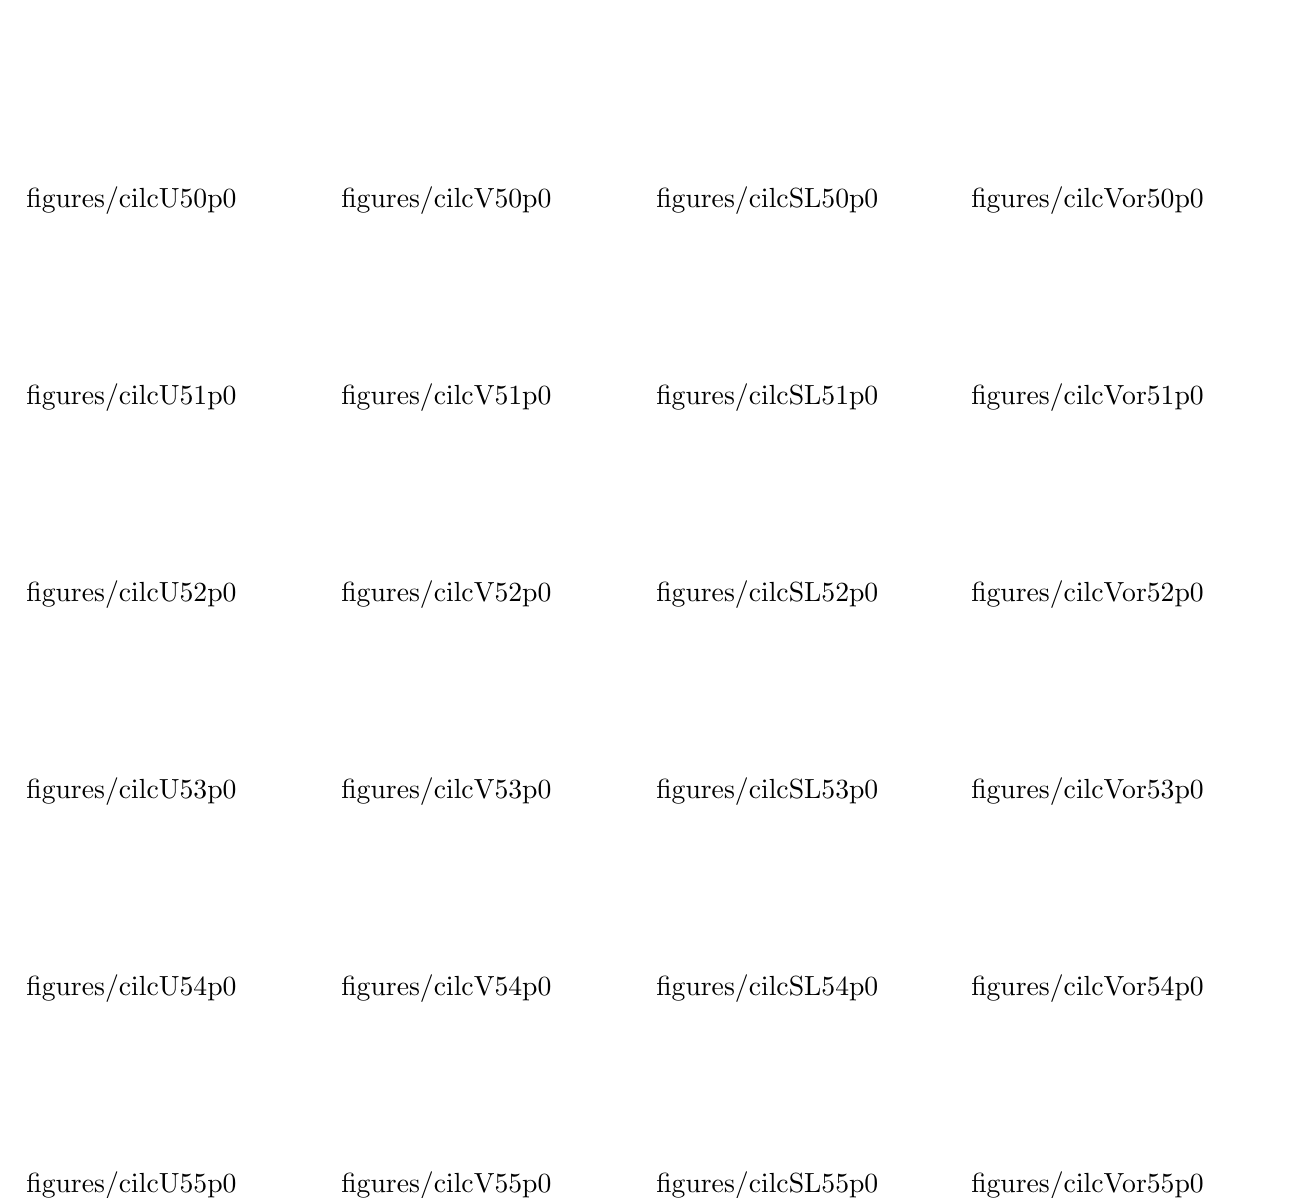
\begin{tikzpicture}[scale=1]
  \useasboundingbox (0,.5) rectangle (16.,15.);  % set the bounding box (so we have less surrounding white space)
  \draw ( 0,12.5) node[anchor=south west,xshift=-4pt,yshift=+0pt] {\trimfig{figures/cilcU50p0}{\figWidth}};
  \draw ( 4,12.5) node[anchor=south west,xshift=-4pt,yshift=+0pt] {\trimfig{figures/cilcV50p0}{\figWidth}};
  \draw ( 8,12.5) node[anchor=south west,xshift=-4pt,yshift=+0pt] {\trimfig{figures/cilcSL50p0}{\figWidth}};
  \draw (12,12.5) node[anchor=south west,xshift=-4pt,yshift=+0pt] {\trimfig{figures/cilcVor50p0}{\figWidth}};
%
  \draw ( 0,10) node[anchor=south west,xshift=-4pt,yshift=+0pt] {\trimfig{figures/cilcU51p0}{\figWidth}};
  \draw ( 4,10) node[anchor=south west,xshift=-4pt,yshift=+0pt] {\trimfig{figures/cilcV51p0}{\figWidth}};
  \draw ( 8,10) node[anchor=south west,xshift=-4pt,yshift=+0pt] {\trimfig{figures/cilcSL51p0}{\figWidth}};
  \draw (12,10) node[anchor=south west,xshift=-4pt,yshift=+0pt] {\trimfig{figures/cilcVor51p0}{\figWidth}};
%
  \draw ( 0,7.5) node[anchor=south west,xshift=-4pt,yshift=+0pt] {\trimfig{figures/cilcU52p0}{\figWidth}};
  \draw ( 4,7.5) node[anchor=south west,xshift=-4pt,yshift=+0pt] {\trimfig{figures/cilcV52p0}{\figWidth}};
  \draw ( 8,7.5) node[anchor=south west,xshift=-4pt,yshift=+0pt] {\trimfig{figures/cilcSL52p0}{\figWidth}};
  \draw (12,7.5) node[anchor=south west,xshift=-4pt,yshift=+0pt] {\trimfig{figures/cilcVor52p0}{\figWidth}};
%
  \draw ( 0, 5) node[anchor=south west,xshift=-4pt,yshift=+0pt] {\trimfig{figures/cilcU53p0}{\figWidth}};
  \draw ( 4, 5) node[anchor=south west,xshift=-4pt,yshift=+0pt] {\trimfig{figures/cilcV53p0}{\figWidth}};
  \draw ( 8, 5) node[anchor=south west,xshift=-4pt,yshift=+0pt] {\trimfig{figures/cilcSL53p0}{\figWidth}};
  \draw (12, 5) node[anchor=south west,xshift=-4pt,yshift=+0pt] {\trimfig{figures/cilcVor53p0}{\figWidth}};
%
  \draw ( 0,2.5) node[anchor=south west,xshift=-4pt,yshift=+0pt] {\trimfig{figures/cilcU54p0}{\figWidth}};
  \draw ( 4,2.5) node[anchor=south west,xshift=-4pt,yshift=+0pt] {\trimfig{figures/cilcV54p0}{\figWidth}};
  \draw ( 8,2.5) node[anchor=south west,xshift=-4pt,yshift=+0pt] {\trimfig{figures/cilcSL54p0}{\figWidth}};
  \draw (12,2.5) node[anchor=south west,xshift=-4pt,yshift=+0pt] {\trimfig{figures/cilcVor54p0}{\figWidth}};
%
  \draw ( 0, 0.) node[anchor=south west,xshift=-4pt,yshift=+0pt] {\trimfig{figures/cilcU55p0}{\figWidth}};
  \draw ( 4, 0.) node[anchor=south west,xshift=-4pt,yshift=+0pt] {\trimfig{figures/cilcV55p0}{\figWidth}};
  \draw ( 8, 0.) node[anchor=south west,xshift=-4pt,yshift=+0pt] {\trimfig{figures/cilcSL55p0}{\figWidth}};
  \draw (12, 0.) node[anchor=south west,xshift=-4pt,yshift=+0pt] {\trimfig{figures/cilcVor55p0}{\figWidth}};
%
 % \draw (current bounding box.south west) rectangle (current bounding box.north east);
% grid:
%  \draw[step=1cm,gray] (0,0) grid (16,15);
\end{tikzpicture}
\end{center}
  \caption{Flow past a cylinder: $u$, $v$, streamlines and vorticity at times $50$, $51$, ... $55$.}
  \label{fig:cylinderSolution}
\end{figure}


\begin{figure}[hbt]
\newcommand{\figWidth}{4cm}
\newcommand{\trimfig}[2]{\trimFig{#1}{#2}{0.0}{.4}{.65}{.55}}
\begin{center}
\begin{tikzpicture}[scale=1]
  \useasboundingbox (0,.5) rectangle (16.,15.);  % set the bounding box (so we have less surrounding white space)
%
  \draw ( 0,10) node[anchor=south west,xshift=-4pt,yshift=+0pt] {\trimfig{figures/cilcPODu0}{\figWidth}};
  \draw ( 4,10) node[anchor=south west,xshift=-4pt,yshift=+0pt] {\trimfig{figures/cilcPODv0}{\figWidth}};
%   \draw ( 8,10) node[anchor=south west,xshift=-4pt,yshift=+0pt] {\trimfig{figures/cilcSL51p0}{\figWidth}};
%   \draw (12,10) node[anchor=south west,xshift=-4pt,yshift=+0pt] {\trimfig{figures/cilcVor51p0}{\figWidth}};
%
  \draw ( 0,7.5) node[anchor=south west,xshift=-4pt,yshift=+0pt] {\trimfig{figures/cilcPODu1}{\figWidth}};
  \draw ( 4,7.5) node[anchor=south west,xshift=-4pt,yshift=+0pt] {\trimfig{figures/cilcPODv1}{\figWidth}};
%   \draw ( 8,7.5) node[anchor=south west,xshift=-4pt,yshift=+0pt] {\trimfig{figures/cilcSL52p0}{\figWidth}};
%   \draw (12,7.5) node[anchor=south west,xshift=-4pt,yshift=+0pt] {\trimfig{figures/cilcVor52p0}{\figWidth}};
%
  \draw ( 0, 5) node[anchor=south west,xshift=-4pt,yshift=+0pt] {\trimfig{figures/cilcPODu2}{\figWidth}};
  \draw ( 4, 5) node[anchor=south west,xshift=-4pt,yshift=+0pt] {\trimfig{figures/cilcPODv2}{\figWidth}};
%   \draw ( 8, 5) node[anchor=south west,xshift=-4pt,yshift=+0pt] {\trimfig{figures/cilcSL53p0}{\figWidth}};
%   \draw (12, 5) node[anchor=south west,xshift=-4pt,yshift=+0pt] {\trimfig{figures/cilcVor53p0}{\figWidth}};
%
  \draw ( 0,2.5) node[anchor=south west,xshift=-4pt,yshift=+0pt] {\trimfig{figures/cilcPODu3}{\figWidth}};
  \draw ( 4,2.5) node[anchor=south west,xshift=-4pt,yshift=+0pt] {\trimfig{figures/cilcPODv3}{\figWidth}};
%   \draw ( 8,2.5) node[anchor=south west,xshift=-4pt,yshift=+0pt] {\trimfig{figures/cilcSL54p0}{\figWidth}};
%   \draw (12,2.5) node[anchor=south west,xshift=-4pt,yshift=+0pt] {\trimfig{figures/cilcVor54p0}{\figWidth}};
%
%  \draw ( 0, 0.) node[anchor=south west,xshift=-4pt,yshift=+0pt] {\trimfig{figures/cilcPODu4}{\figWidth}};
%  \draw ( 4, 0.) node[anchor=south west,xshift=-4pt,yshift=+0pt] {\trimfig{figures/cilcPODv4}{\figWidth}};
%  \draw ( 8, 0.) node[anchor=south west,xshift=-4pt,yshift=+0pt] {\trimfig{figures/cilcSL55p0}{\figWidth}};
%  \draw (12, 0.) node[anchor=south west,xshift=-4pt,yshift=+0pt] {\trimfig{figures/cilcVor55p0}{\figWidth}};
%
 % \draw (current bounding box.south west) rectangle (current bounding box.north east);
% grid:
%  \draw[step=1cm,gray] (0,0) grid (16,15);
\end{tikzpicture}
\end{center}
  \caption{Flow past a cylinder: POD vectors, $u$, $v$.}
  \label{fig:cylinderSolution}
\end{figure}

% -------------------------------------------------------------------------------------------------
\vfill\eject
\bibliography{\homeHenshaw/papers/henshaw}
\bibliographystyle{siam}


\end{document}
